\section{Introduction}\label{sec:introduction}

\begin{wrapfigure}{r}{0.5\textwidth}
    \centering
    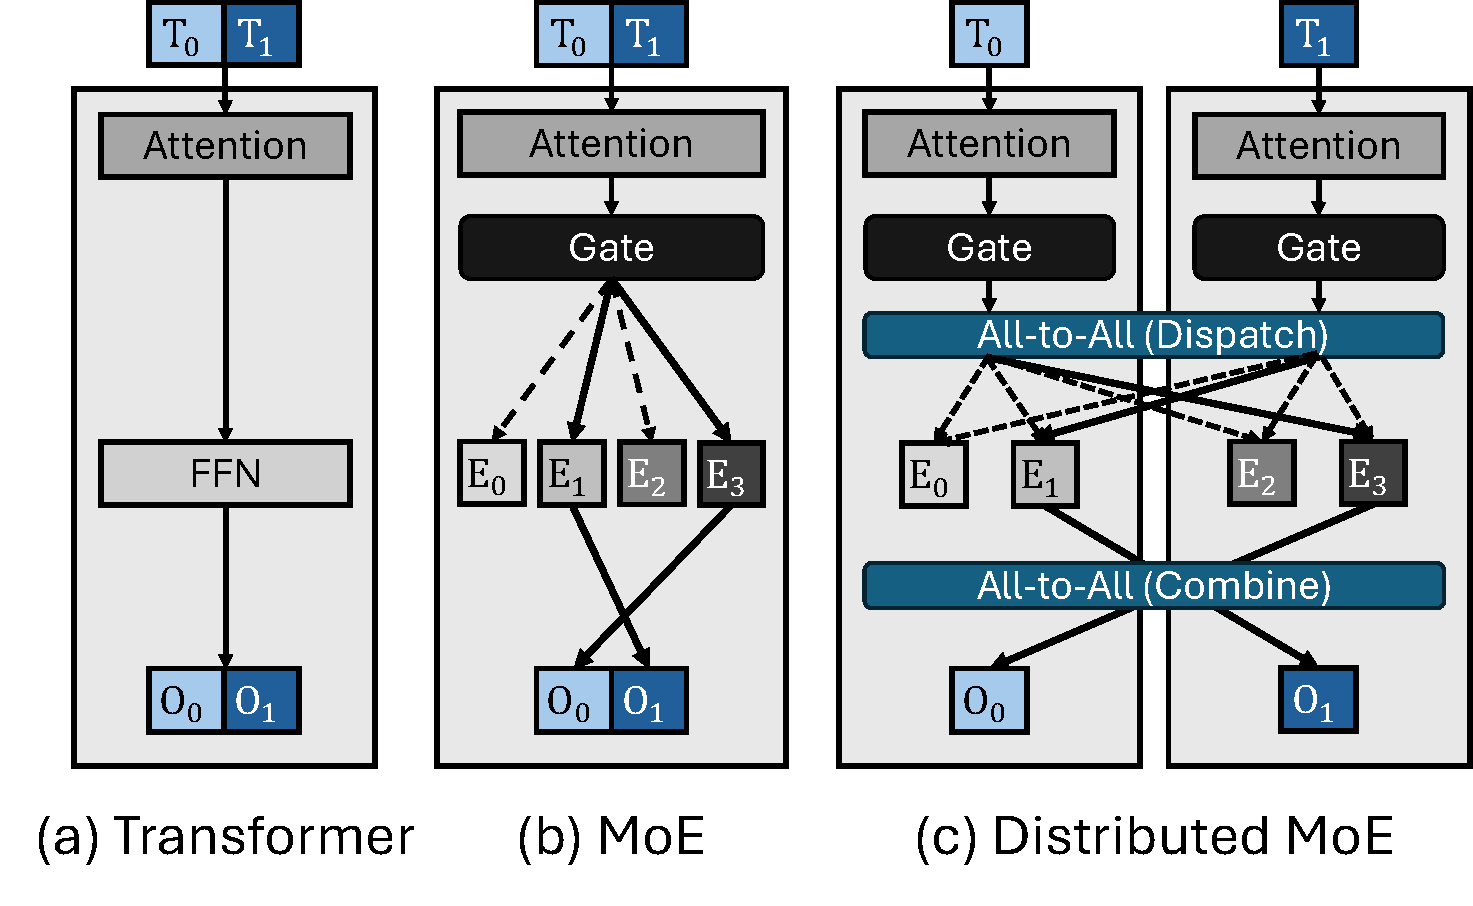
\includegraphics[width=0.51\textwidth, keepaspectratio]{figures/fig-bg-moe}
    \caption{Transformer blocks (a) without MoE, (b) with MoE, and (c) with distributed MoE and expert parallelism.
    \texttt{T}, \texttt{E}, and \texttt{O} represent input tokens, experts, and output activations, respectively.}
    \label{fig:bg:moe}
    \vspace{-10pt}
\end{wrapfigure}

State-of-the-art large language models (LLMs)~\cite{deepep, llama4, dbrx, arctic, openai2025gptoss} have adopted the Mixture-of-Experts (MoE) architecture for its computational efficiency and strong performance across a range of tasks. The traditional Transformer block consists of a self-attention module followed by a dense feed-forward network (FFN)~\cite{NIPS2017_3f5ee243}. In contrast, MoE architectures replace this single FFN (Figure~\ref{fig:bg:moe}(a)) with many identically sized FFNs, known as experts (Figure~\ref{fig:bg:moe}(b)). A trainable neural network, known as a gate function, sparsely activates these experts by dynamically routing input tokens to the experts selected at runtime. This increase in model parameters due to more FFNs improves model quality without the corresponding increase in computational cost.

\myparab{Communication overheads in MoE.}  
As MoE model sizes grow, GPU memory constraints prevent hosting all experts on a single device. The standard practice is to distribute experts across multiple GPUs using expert parallelism (EP), which requires token routing via many-to-many communication primitives like \alltoall~\cite{deepep, arctic, dbrx, 10.1145/3577193.3593704} (Figure~\ref{fig:bg:moe}(c)). Another round of \alltoall communication restores the permuted tokens processed by experts to their original order in the sequence. \alltoall communication is challenging to optimize on GPU networks and is highly sensitive to straggler delays --- a phenomenon where a single straggler GPU delays all others from making progress~\cite{stragglar}. These communication operations can account for 68\% of the total runtime~\cite{10.1145/3603269.3604869, MLSYS2024_339caf45}, causing GPUs to remain idle (Figure~\ref{fig:intro}, top left).


% Existing work has observed these communication operations can take 68\% of total runtime~\cite{10.1145/3603269.3604869, MLSYS2024_339caf45}, during which the GPU is idle, unless the implementation explicitly overlaps with computation.
% To mitigate these communication bottlenecks, recent work pipelines computation with communication tasks (Figure~\ref{fig:intro}, middle left). This form of pipelining is challenging to achieve efficiently because it requires \emph{asynchronous GPU-driven communication} and \emph{kernel fusion} to maximize the overlap efficiency. Typically, inter-GPU communication APIs available in frameworks like PyTorch are not of this kind but instead are \emph{CPU-driven}~\cite{nccl}.

\myparab{Kernel launch overheads in MoE.} 
To mitigate these communication bottlenecks, recent work pipelines computation with communication kernels (Figure~\ref{fig:intro}, left middle). However, the effectiveness of these solutions is limited by the overhead of launching many kernels from the CPU. 
Specifically, existing implementations~\cite{pmlr-v162-rajbhandari22a, comet, megatron, fastermoe} launch a large number of kernels per a single layer pass (see Table~\ref{tab:gpuOps}). Frequent kernel launches negatively affect performance by:
(1) creating non-deterministic kernel start times across GPUs, exacerbating straggler issues; (2) introducing unnecessary synchronization points, causing GPUs to wait on peers or the CPU before proceeding; and (3) incurring repeated global memory round trips at kernel boundaries. Although CUDA graphs~\cite{cuda_graphs_nvidia_blog} can partially mitigate the first issue in static workloads, they are incompatible with MoE's dynamic expert routing patterns. Addressing the remaining issues requires novel solutions,
which we provide in this work through complete kernel fusion and asynchronous device-initiated communication.


\begin{figure}[!ht]
    \centering
    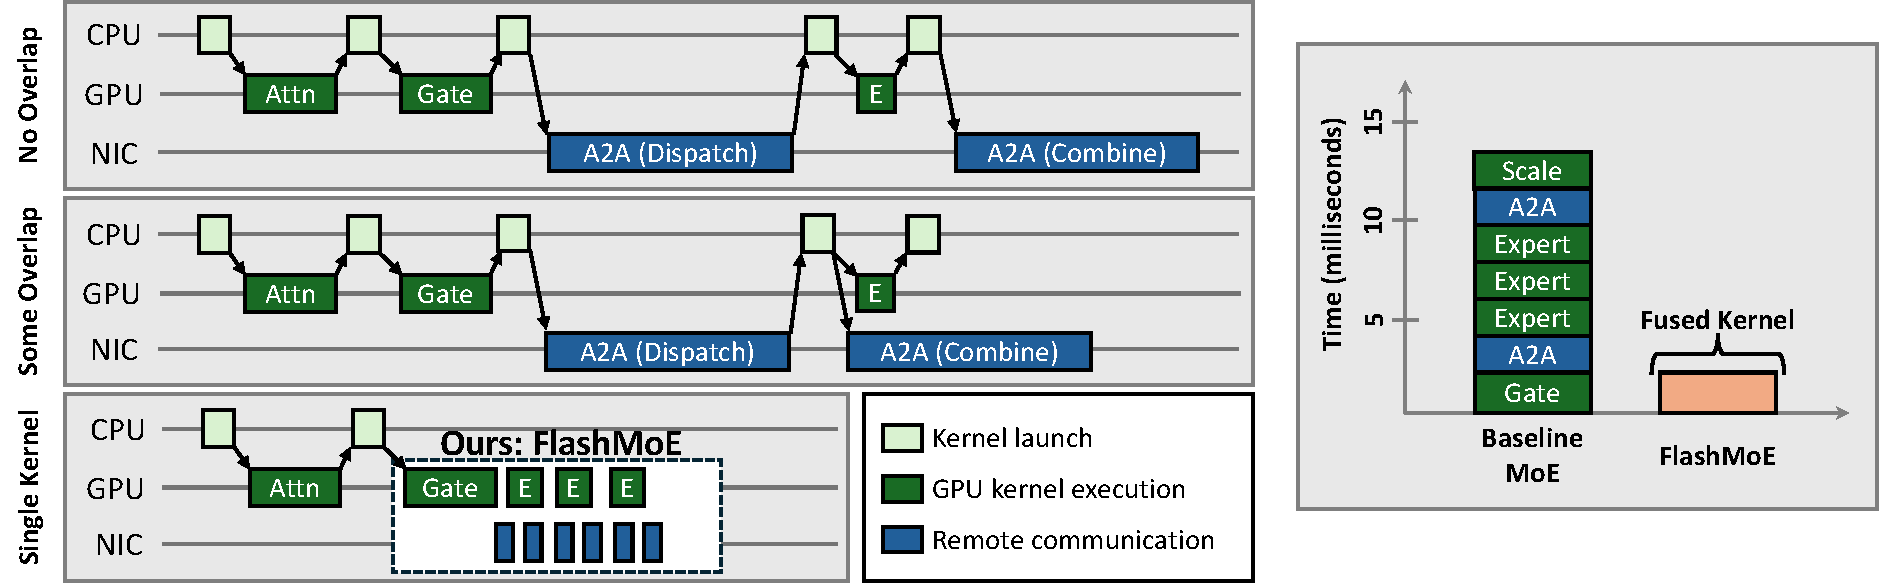
\includegraphics[width=0.98\textwidth, keepaspectratio]{figures/intro-fig}
    \caption{Comparing \sysname with state-of-the-art techniques that either do not overlap communication and computation (left, top) or do some overlap (left, middle). \sysname is a persistent kernel that fuses all computation and communication of the MoE operator (left, bottom). \sysname implements device-initiated computation (gate, expert FFN, scale) and communication tasks (right).}
    \label{fig:intro}
    \vspace{-10pt}
\end{figure}
\begin{table}[!ht]
    \centering
    \small
    \renewcommand{\arraystretch}{0.9}
    \begin{tabular}{@{}lc@{}}
        \toprule
        \textbf{MoE Implementation} & \textbf{Launched GPU Ops} \\ \midrule
        \sysname & 1 \\
        COMET~\cite{comet} & 33 \\
        Megatron-LM CUTLASS~\cite{megatron, 10.1145/3458817.3476209} & 85 \\
        Megatron-LM TE~\cite{megatron, 10.1145/3458817.3476209} & 261 \\
        Megatron-LM + DeepEP~\cite{deepep} & 432 \\
        DeepSpeedMoE~\cite{pmlr-v162-rajbhandari22a} & 550 \\
        \bottomrule
    \end{tabular}
    \vspace{1mm}
    \caption{
    We report number of GPU operations launched by MoE implementations by profiling with Nsight Systems~\cite{nsight-metrics}. We count operations in a single MoE layer (Gate $\rightarrow$ Dispatch $\rightarrow$ Expert $\rightarrow$ Combine) on 2 A100 GPUs, where each GPU has 32 experts. \sysname is the first to fully fuse the distributed MoE layer into a single GPU kernel.}
    \label{tab:gpuOps}
\end{table}
\subsection{Our Contributions: distributed MoE in a single kernel}
To overcome these fundamental inefficiencies in state-of-the-art MoE models, we develop \sysname, where we integrate all MoE computation and communication tasks into a single persistent GPU kernel
\ie a kernel that remains active for the entirety of the MoE operator (Figure~\ref{fig:intro} bottom left).
Instead of multiple kernel launches coordinated by the CPU, \sysname requires launching only one kernel,
significantly reducing the involvement of the CPU\@.
Within the fused kernel, \sysname implements a reactive programming model to achieve
fine-grained parallelism and loosely coupled, non-blocking execution among tens of thousands of GPU threads.

\myparab{In-kernel Block scheduling and Tile parallelism.}
\sysname implements \emph{tile-level parallelism},
meaning it partitions input token matrices into smaller, independent units called \emph{tiles},
which are processed by blocks but managed (scheduled and constructed) by warps.
We specialize every thread block, except one, as \emph{processors} to perform compute.
In addition, we designate a dedicated Operating System (OS) block (4 warps) to perform administrative tasks of
(1) scheduling computational work to processors (\emph{scheduler}),
and (2) decoding computational tasks from messages received from other GPUs (\emph{subscriber}).
This design allows \sysname to dynamically assign tasks to GPU blocks based on \emph{readiness},
ensuring that no GPU SM remains idle throughout the lifetime of the MoE operator.
\sysname selects tile dimensions to maximize GPU arithmetic intensity
while still benefitting from a high-degree of parallelism.

\myparab{Asynchronous and payload-efficient communication.}
By redesigning the MoE operator from the ground up,
\sysname resolves fundamental inefficiencies inherent in the conventional MoE execution pipeline.
One notable inefficiency is token padding during communication.
To simplify programming complexity and due to symmetry constraints of collective communication APIs,
existing implementations have to zero-pad token payloads to match predefined buffer sizes.
This occurs when tokens are asymmetrically routed to experts, resulting in GPUs receiving much less than the expected
capacity.
However, these null payloads waste communication bandwidth, bloat data transfer latency and may lead to
unnecessary computations on null matrices in some implementations.
\sysname introduces \emph{payload-efficient} communication by sending non-padded tokens only to
GPUs with actively selected experts, conserving both communication and computational resources.

\myparab{Technical challenges.}
Realizing the single-kernel design of \sysname required
solving several technical challenges to achieve high performance:
(1) lightweight computational dependency management; (2)
navigating optimal SM occupancy configurations; (3) implementing in-device BLAS operations;
(4) minimizing inter- and intra-device synchronization overheads; (5) implementing transfer-awareness by leveraging
DMA over Unified Virtual Addressing (UVA) when available.
In addressing these challenges, \sysname's design presents a
radical departure from traditional synchronous \alltoall collectives,
where GPUs exhibit significant idle time during layer execution.
For device-initiated communication,
\sysname uses NVSHMEM~\cite{nvshm} to establish a global address space across all GPUs to
achieve the aforementioned Direct Memory Access (DMA) or Remote DMA (RDMA) communication.
For in-device BLAS, \sysname develops custom high-performance GEMM operations via CUTLASS~\cite{Thakkar_CUTLASS_2023}.

\myparab{Results.}
We evaluate \sysname across multiple GPUs split across multiple nodes.
Our evaluations show that \sysname achieves \textbf{6}$\times$ latency speedup,
\textbf{9}$\times$ higher GPU utilization, \textbf{4}$\times$ better weak scaling efficiency and \textbf{5.7}$\times$
increased throughput compared to state-of-the-art implementations.
We project these performance gains becoming even better in multi-node scenarios,
where inter-node communication occurs using lower bandwidth inter-node links (\eg RDMA, Infiniband).
